
\documentclass[submit]{harvardml}

% Put in your full name and email address.
\name{Weiyi Chen}
\email{wec427@g.harvard.edu}

% List any people you worked with.
\collaborators{%
}

% You don't need to change these.
\course{CS181-S16}
\assignment{Assignment \#3}
\duedate{March 27, 2016}

\usepackage[OT1]{fontenc}
\usepackage[colorlinks,citecolor=blue,urlcolor=blue]{hyperref}
\usepackage[pdftex]{graphicx}
\usepackage{subfig}
\usepackage{fullpage}
\usepackage{palatino}
\usepackage{mathpazo}
\usepackage{amsmath}
\usepackage{amssymb}
\usepackage{color}
\usepackage{todonotes}
\usepackage{listings}
\usepackage{common}
\usepackage{bm}

\usepackage[mmddyyyy,hhmmss]{datetime}

\definecolor{verbgray}{gray}{0.9}

\lstnewenvironment{csv}{%
  \lstset{backgroundcolor=\color{verbgray},
  frame=single,
  framerule=0pt,
  basicstyle=\ttfamily,
  columns=fullflexible}}{}

\begin{document}
\begin{center}
{\Large Homework 3: SVM}\\
\end{center}

There is a mathematical component and a programming component to this homework.
Please submit ONLY your PDF to Canvas, and push all of your work to your Github
repository. If a question asks you to make any plots, like Problem 3, please
include those in the writeup.

%%%%%%%%%%%%%%%%%%%%%%%%%%%%%%%%%%%%%%%%%%%%%
% Problem 1
%%%%%%%%%%%%%%%%%%%%%%%%%%%%%%%%%%%%%%%%%%%%%
\begin{problem}[Fitting an SVM by hand, 8pts]
Consider a dataset with the following 6 points in $1D$: \[\{(x_1, y_1)\} =\{(-3
, +1 ), (-2 , +1 ) , (-1,  -1 ), ( 1 , -1 ), ( 2 , +1 ), ( 3 , +1 )\}\] Consider
mapping these points to $2$ dimensions using the feature vector $\phi : x
\mapsto (x, x^2)$. The max-margin classifier objective is given by:
\begin{equation}
  \min_{\mathbf{w}, w_0} \|\mathbf{w}\|_2^2 \quad \text{s.t.} \quad y_i(\mathbf{w}^T \phi(x_i) +
  w_0) \geq 1,~\forall i
\end{equation}

Note: the purpose of this exercise is to solve the SVM without the help of a
computer, relying instead on principled rules and properties of these
classifiers. The exercise has been broken down into a series of questions, each
providing a part of the solution. Make sure to follow the logical structure of
the exercise when composing your answer and to justify each step.

\begin{enumerate}
  \item Write down a vector that is parallel to the optimal vector $\mathbf{w}$. Justify
    your answer.
  \item What is the value of the margin achieved by $\mathbf{w}$? Justify your
    answer.
  \item Solve for $\mathbf{w}$ using your answers to the two previous questions.
  \item Solve for $w_0$. Justify your answer.
  \item Write down the discriminant as an explicit function of $x$.
\end{enumerate}

\end{problem}
\subsection*{Solution}

\begin{figure}
    \centering
    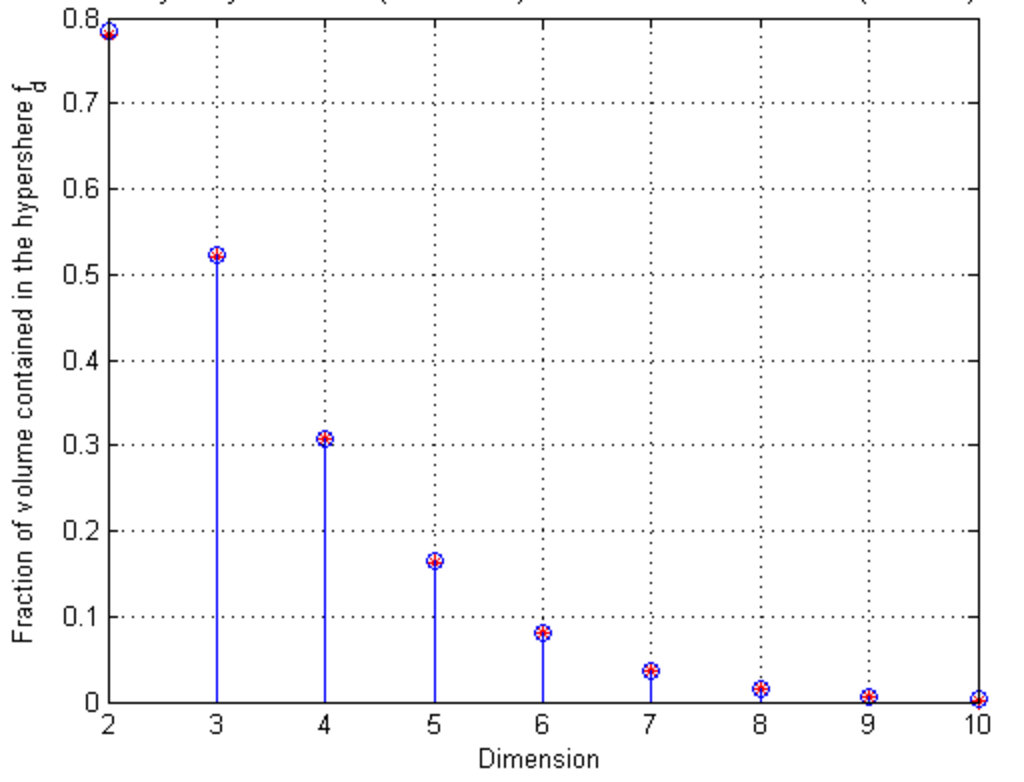
\includegraphics[scale=0.3]{prob1.png}
    \caption{Plot of 6 points using the feature vectors}
\end{figure}

\begin{enumerate}
  \item A vector that is parallel to the optimal vector $\mathbf{w}$ is $\mathbf{w}'^T = (0,1)$.
  
  To justify it, see the plot on the next page. We plot the feature vectors and obviously there are 4 points in $+1$ class as of $$(-3,9),(-2,4),(2,4),(3,9)$$ and the other 2 points in the $-1$ class as of $$(-1,1), (1,1)$$
  
  Obviously the support vectors are $(-2,4), (2,4)$ for $y=+1$ class and $(-1,1), (1,1)$ for $y=-1$ class. Also according to the symmetry and parallelity of the points, a max-margin boundary is obviously parallel to the x-axis and in the middle of those 4 support vectors (indicated as the dash line). $\mathbf{w}$ is perpendicular to the decision boundary between the support vectors in the 2d feature space, therefore $\mathbf{w}'^T = (0,1)$ which is perpendicular to the dash line should be parallel to the optimal vector.
  
  \item The value of the margin achieved by $\mathbf{w}$ is $1.5$.
  
  To justify it, recall that the margin is the distance from each support vector to the decision boundary. From the geometry plot above, with 4 points being support vectors, with a dash line separating two from the other two paralleled. The margin is just a half of the perpendicular distance between two points from different side, as of
  $$ \frac{1}{||\mathbf{w}||_2} = (4 - 1) / 2 = 1.5 $$
  
  \item Given the conclusion of part 2 using the fact the margin is $\frac{1}{||\mathbf{w}||_2}$, we have 
  $$ ||\mathbf{w}||_2 = \frac{2}{3} $$
  And given the conclusion of part 1 that the unit vector of $\mathbf{w}$ is $\mathbf{w}'^T=(0,1)$, we derive

  $$ \mathbf{w}^T = (0, \frac{2}{3}) $$
  
  \item To solve $w_0$, we can just substitute any of the support vectors into the formula $y_i(\mathbf{w}^T\phi(x_i) + w_0) = 1$ where $\mathbf{w}^T$ has been solved in the last part, we derive $$w_0=-\frac{5}{3}$$. To justify this, the points are on the decision boundary, so the inequalities will be tight. A “tight inequality” is an inequality that is as strict as possible. For this problem, this means that plugging in these points will push the left-hand side of Equations (1) as close to $1$ as possible.
  
  \item Write down the form of the discriminant function 
  $$ f(x) = w_0+ \mathbf{w}^T \phi(x) $$ as an explicit function
  of x, by substituting $\mathbf{w}^T$ and $w_0$, we have
  $$ f(x) = -\frac{5}{3} + \frac{2}{3}x^2 $$
  
\end{enumerate}


\newpage
%%%%%%%%%%%%%%%%%%%%%%%%%%%%%%%%%%%%%%%%%%%%%
% Problem 2
%%%%%%%%%%%%%%%%%%%%%%%%%%%%%%%%%%%%%%%%%%%%%
\begin{problem}[Composing Kernel Functions , 7pts]
Prove that
\begin{align*}
	K(\boldx, \boldx') &= \exp\{ -||\boldx - \boldx'||^2_2 \}\,,
\end{align*}
where~$\boldx,\boldx'\in\reals^D$ is a valid kernel, using only the following
properties.  If~$K_1(\cdot,\cdot)$ and~$K_2(\cdot,\cdot)$ are valid kernels,
then the following are also valid kernels:
\begin{align*}
	K(\boldx, \boldx') &= c\,K_1(\boldx, \boldx') \quad \text{for $c>0$}\\
	K(\boldx, \boldx') &= K_1(\boldx, \boldx') + K_2(\boldx, \boldx')\\
	K(\boldx, \boldx') &= K_1(\boldx, \boldx')\,K_2(\boldx, \boldx')\\
	K(\boldx, \boldx') &= \exp\{ K_1(\boldx, \boldx') \}\\
  K(\boldx, \boldx') &= f(\boldx)\,K_1(\boldx, \boldx')\,f(\boldx') \quad
  \text{where $f$ is any function from~$\reals^D$ to $\reals$}
\end{align*}

 \end{problem}
\subsection*{Solution}

Let's look at the given kernel
$$ K(\boldx,\boldx') = \exp({-||\boldx - \boldx'||^2_2})
 = \exp(-\boldx^T\boldx)\exp(\boldx^T\boldx')\exp(-\boldx'^T\boldx') $$

According to formula 5 where
$$ f(\boldx) = \exp(-\boldx^T\boldx), f(\boldx') = \exp(-\boldx'^T\boldx') $$
we only need to prove that $exp(\boldx^T\boldx')$ is a valid kernel.

According to formula 4 where 
$$ K_1(\boldx, \boldx') = \boldx^T\boldx'$$
we then further reduce only need to prove that $\boldx^T\boldx'$ is a valid kernel. 

Obviously $\boldx^T\boldx'$ is just an inner product, we have $\boldx^T\boldx'$ is a valid kernel, thus $K(\boldx, \boldx') = \exp\{ -||\boldx - \boldx'||^2_2 \}$ is a valid kernel.

\newpage
%%%%%%%%%%%%%%%%%%%%%%%%%%%%%%%%%%%%%%%%%%%%%
% Problem 3
%%%%%%%%%%%%%%%%%%%%%%%%%%%%%%%%%%%%%%%%%%%%%
\begin{problem}[Scaling up your SVM solver, 10pts (+7pts with extra credit)]



In the previous homework, you studied a simple data set of fruit measurements.
We would like you to code up a few simple SVM solvers to classify lemons from
apples. To do this, read the paper at
\url{http://www.jmlr.org/papers/volume6/bordes05a/bordes05a.pdf} and implement
the Kernel Perceptron algorithm and the Budget Kernel Perceptron algorithm. The provided code has a base Perceptron class, which you will inherit to write KernelPerceptron and BudgetKernelPerceptron. This has been set up for you in problem3.py. The provided data is linearly separable. Make the optimization as fast as
possible. 

Additionally, we would like you to do some experimentation with the hyperparameters for each of these models. Try seeing if you can identify some patterns by changing $\beta$, N (maximum number of support vectors), or the number of random samples you take.  Note the training time, accuracy,  shapes/orientations of hyperplanes, and number of support vectors for various setups. We are intentionally leaving this open-ended to allow for experimentation, and so we will be looking for your thought process and not a rigid graph this time. That being said, any visualizations that you want us to grade and refer to in your descriptions should be included in this writeup. You can use the trivial $K(\mathbf{x_1}, \mathbf{x_2}) = \mathbf{x_1}^T\mathbf{x_2}$ kernel for this problem, though you are welcome to experiment with more interesting kernels too. Also, answer the following reading questions in one or two sentences each.

\begin{enumerate}
\item In one short sentence, state the main purpose of the paper?
\item Identify each of the parameters in Eq. 1
\item State one guarantee for the Kernel perceptron algorithm described in the
  paper.
\item What is the main way the budget kernel perceptron algorithm tries to
  improve on the perceptron algorithm.
\item In simple words, what is the theoretical guarantee of LASVM algorithm? How
  does it compare to its practical performance?
\end{enumerate}


For extra credit (+7 pts), implement the SMO algorithm and implement the LASVM process and do the same as above.




\end{problem}

\subsection*{Solution}

\begin{enumerate}
  \item The main purpose of the paper is to propose empirically that, efficient learning algorithm usually takes a brief look at training examples (LASVM vs. SVM), and example selection is also essential to further optimize with less memory, faster speed and higher accuracy.
  
  \item Eq.1 is given by
  $$ \hat y(x) = w' \Phi(x) + b $$
  where $x$ corresponds to pattern, $\Phi(x)$ corresponds to the feature vectors which are the first two columns in "data.csv", $y(x)$ is the class/response of the data which corresponds to the third column in "data.csv", and it also represents the prediction of test data as it is noted $\hat y(x)$. 
  
  $w$ and $b$ are parameters to decide decision boundary, and they are determined by running some learning algorithm on a set of training examples. In the paper/our practice, especially for the "Kernel Perceptron" and "Budget Kernel Perceptron", $b$ is set to zero, parameter vector $w$ can be expressed as a linear combinations of the training patters as of
  
  $$ w = \sum_i^n = \alpha_i \Phi(x_i) $$ 
  
  \item One obvious guarantee is that Kernel perceptron algorithm requires very little memory because the examples are processed one by one and can be discarded after being examined.
  
  Another more important guarantee of accuracy is that iterations such that $y_t\hat y(x_t) < 0$ are called mistakes because they correspond to patterns misclassified by the perceptron decision boundary. The algorithm then modifies the decision boundary by inserting the misclassified pattern into the kernel expansion. When a solution exists, Novikoff’s Theorem states that the algorithm converges after a finite number of mistakes, or equivalently after inserting a finite number of support vectors.
  
  \item The main way the budget kernel perceptron algorithm improves on the perceptron algorithm is add a removal step on the support vectors from the kernel expansion. This makes it perform nicely on relatively clean data sets.
  
  \item The theoretical guarantee of LASVM algorithm is it is a reorganization of the SMO sequential direction searches and converges to the SVM QP problem. It also sports a support vector removal step, which idea is similar to Budget Kernel, that is vectors collected in the current kernel expansion can be removed during the online process.
  
  Compared to its practical performance, LASVM features a removal step and gracefully handles noisy data compared to the kernel perceptrons, it converges to known SVM solution which has theoretical guarantee compared to budget kernel, and it bring the computational benefits and the flexibility of online learning algorithms compared to a traditional SVM solver. Also the practical evidence shows that LASVM matches the SVM accuracy after a single sequestial pass over the training examples. LASVM reliably reaches competitive accuracies after performing a single pass over the training examples, outspeeding state-of-the-art SVM solvers.
  
\end{enumerate}

\subsection*{Experiments}
The github link is \url{https://github.com/harvard-ml-courses/cs181-s16-homework1-weiyialanchen/tree/master/homework3}.

\subsubsection*{Implementation of Kernel Perceptron}
The Kernel Perceptron algorithm is implemented and generates visualization plot as of Figure 2.
 
 \begin{figure}
     \centering
     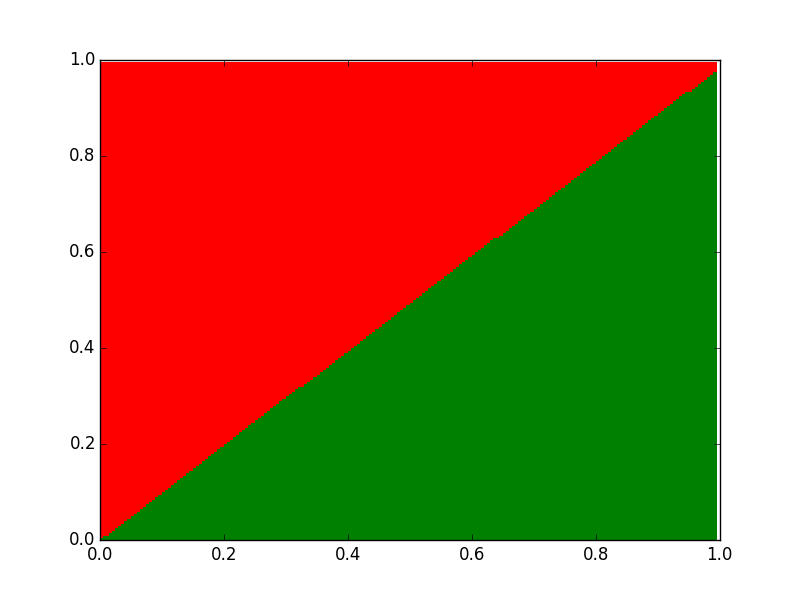
\includegraphics[scale=0.3]{k.png}
     \caption{Plot of Kernel Perceptron}
 \end{figure}

which is expected and matched to the data point plot. (Note it's not a perfect diagonal boundary because I only trained on a subset of data in order to speed up the experiments, and this is not a big matter since it's almost reaching the truth even with a small set of random data.

\subsubsection*{Implementation of Budget Kernel Perceptron}

The Budget Kernel is only slightly different from the basic Kernel, so I derive this Perceptron class from the basic kernel perceptron and override the "fit" method. The initial plot generated is Figure 3.

 \begin{figure}
     \centering
     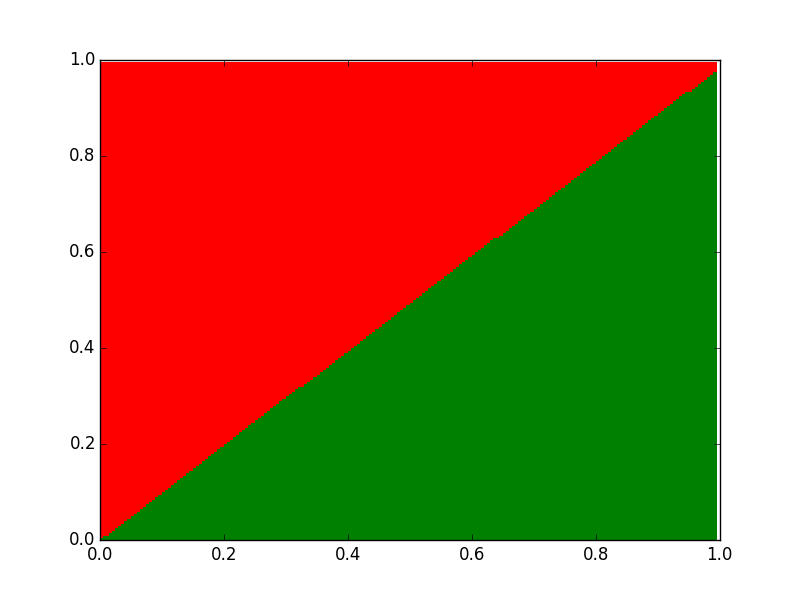
\includegraphics[scale=0.3]{bk.png}
     \caption{Plot of Budget Kernel Perceptron}
 \end{figure}

It still works well, actually exactly the same as the basic perceptron. This is because I trained a dataset of 1000 points, and only "77 support vectors out of 1000 points" (output of my program) are required. As $beta=0$ and $N=100$ initially, this run is exactly the same as the basic kernel (the constraint does not contribute), but this is a good start to verify.

\subsubsection*{Adjustment of $N$}

Let's change $N$ in Budget Kernel Perceptron to make it smaller than $77$ and see what happens. When $N=75$, see Figure 4, it does not affect anything (or can be ignored) since removing those 1 or 2 support vectors does not influence the performance of Budget Kernel. 

 \begin{figure}
     \centering
     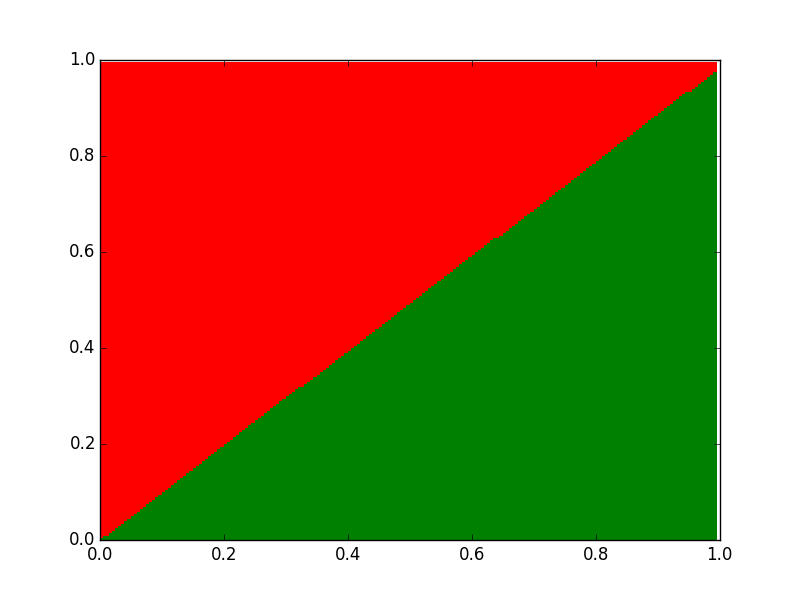
\includegraphics[scale=0.3]{bk.png}
     \caption{Plot of Budget Kernel Perceptron with $N=75$}
 \end{figure}

But if we keep decreasing to $N=60, 45, 30$, the plot are generated as Figure 5, Figure 6 and Figure 7.

 \begin{figure}
     \centering
     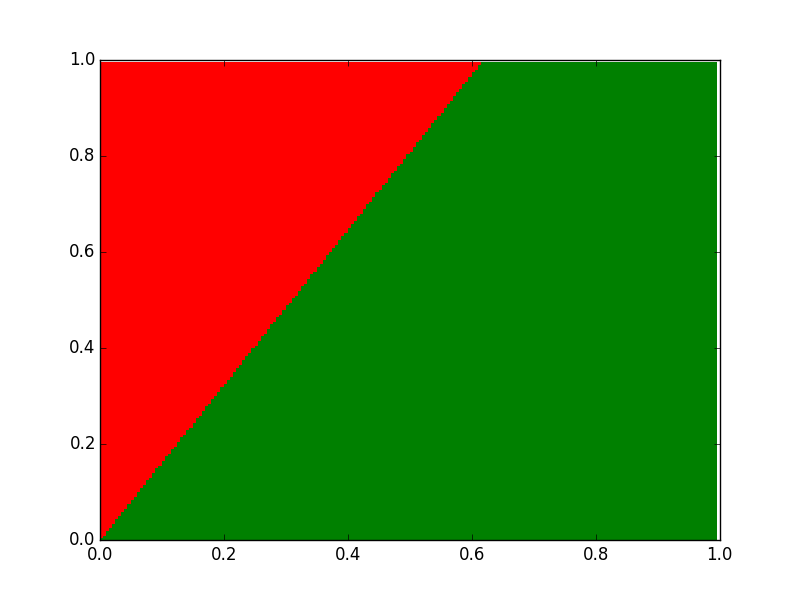
\includegraphics[scale=0.3]{bk-N76.png}
     \caption{Plot of Budget Kernel Perceptron with $N=60$}
 \end{figure}
 
  \begin{figure}
     \centering
     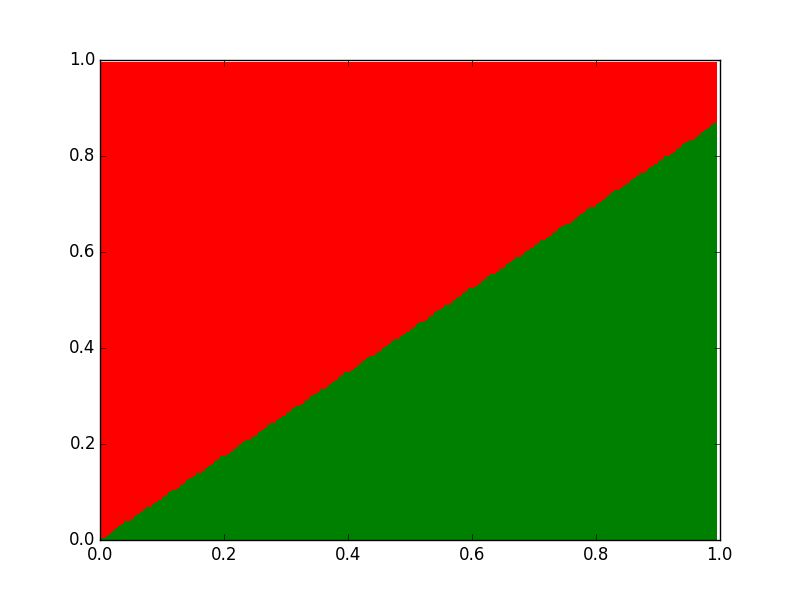
\includegraphics[scale=0.3]{bk-N75.png}
     \caption{Plot of Budget Kernel Perceptron with $N=45$}
 \end{figure}
 
  \begin{figure}
     \centering
     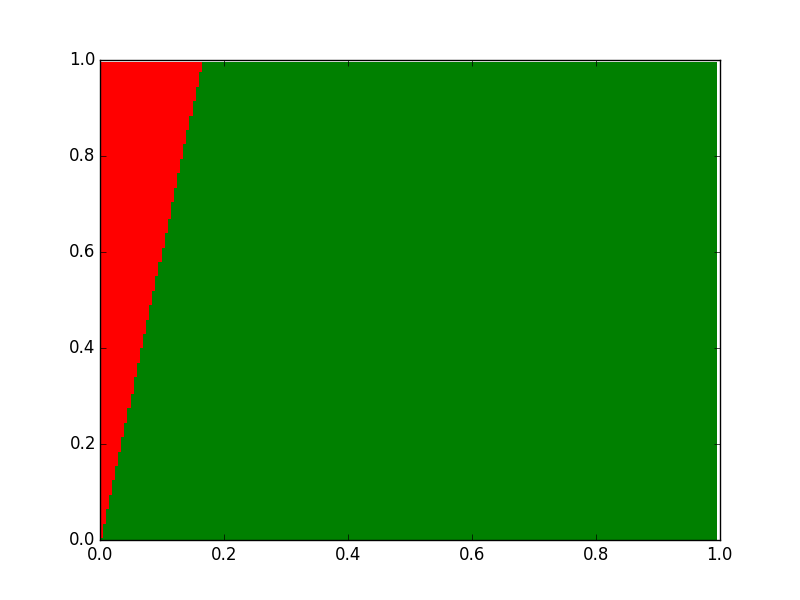
\includegraphics[scale=0.3]{bk-N74.png}
     \caption{Plot of Budget Kernel Perceptron with $N=30$}
 \end{figure}

Though the program speeds up more and more, the boundary also becomes farther and farther to the truth diagonal line, which is caused by the constraint of maximum support vectors. The support vectors are not enough, and some of the essential ones are removed as well, which makes it very weird. 

\subsubsection*{Adjustment of $\beta$}

Adjustment on $\beta$ is similar to $N$, but just a different parameter to control. Let's revert $N=100$, and adjust $\beta$ slightly. Figure 8, 9, 10 are the plots with $\beta=0.1, 0.15, 0.2$,

 \begin{figure}
     \centering
     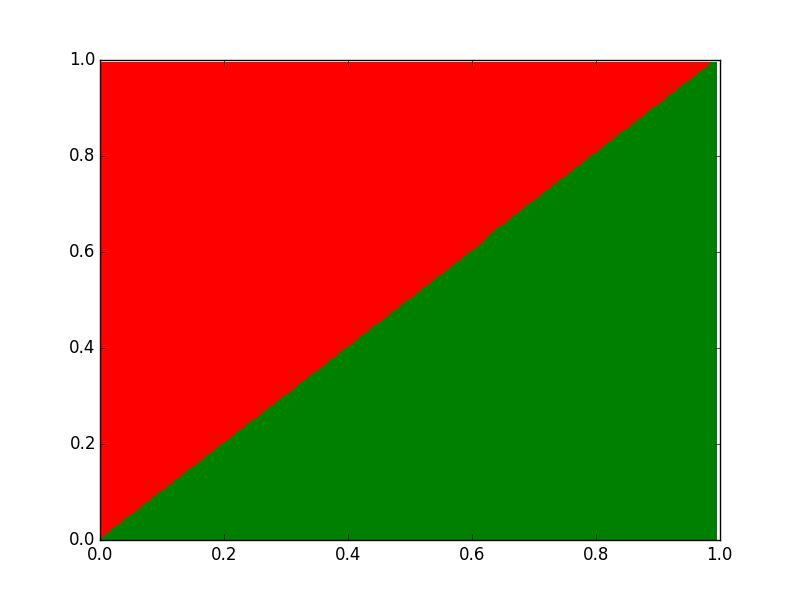
\includegraphics[scale=0.3]{bk-beta01.png}
     \caption{Plot of Budget Kernel Perceptron with $\beta=0.1$}
 \end{figure}
 
  \begin{figure}
     \centering
     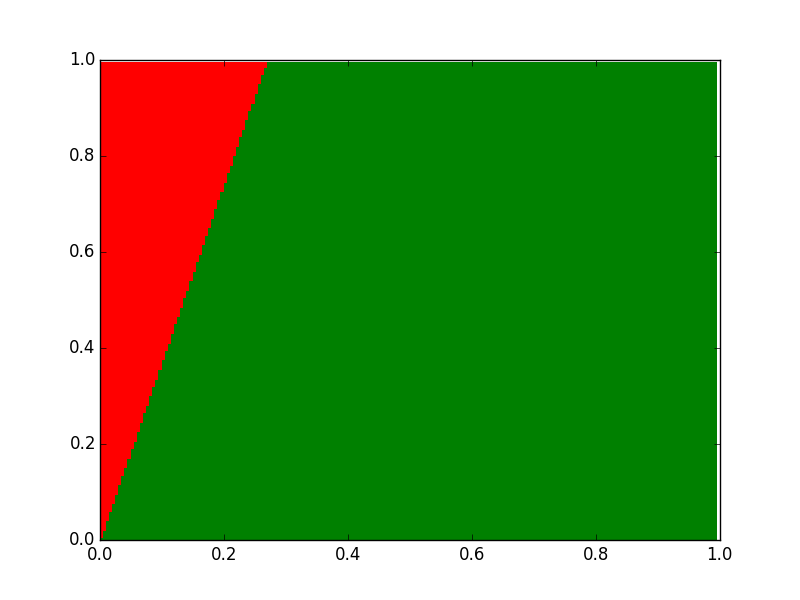
\includegraphics[scale=0.3]{bk-beta014.png}
     \caption{Plot of Budget Kernel Perceptron with $\beta=0.15$}
 \end{figure}
 
  \begin{figure}
     \centering
     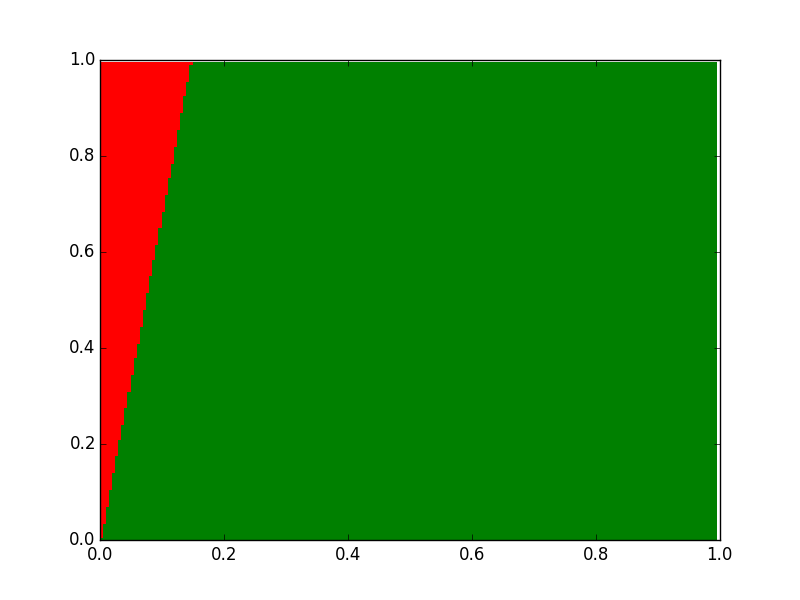
\includegraphics[scale=0.3]{bk-beta015.png}
     \caption{Plot of Budget Kernel Perceptron with $\beta=0.2$}
 \end{figure}

One thing need to note is that when $\beta$ is changed, the number of final support vectors (output of my program) is changed too, i.e. 77, 98, 100 support vectors in these three plots. So actually $N$ starts to have effect again when $\beta$ increases. Therefore in practice, these two parameters should be adjusted together.

\subsubsection*{Extra credits}

I have also implemented the SMO algorithm and the LASVM process, please refer to the Github. The result of of them are almost the same since the data are linearly separable, and the speed of SMO and LASVM are faster than basic perceptron and budget perceptron in general. Their plot are exactly the same with perfect boundary as of the diagonal line, see Plot 11.

  \begin{figure}
     \centering
     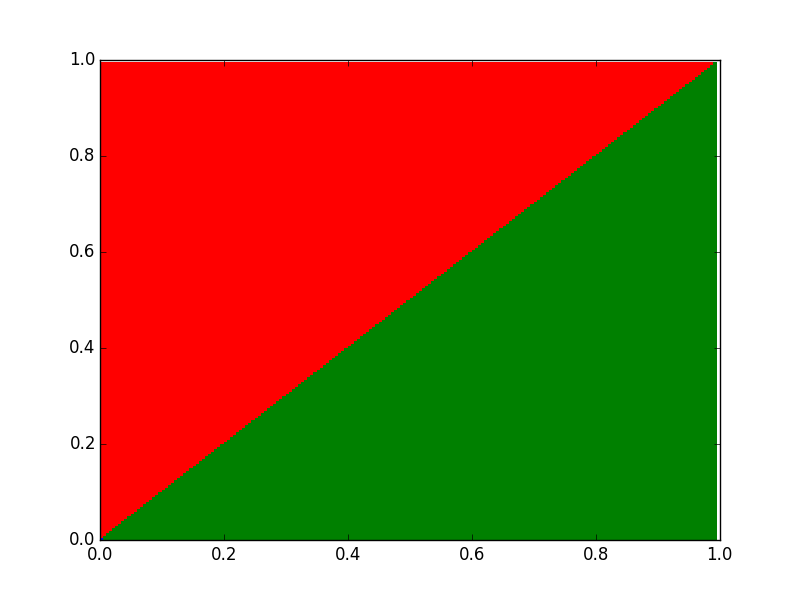
\includegraphics[scale=0.3]{smo.png}
     \caption{Plot of SMO and LASVM}
 \end{figure}

\newpage

\subsection*{Calibration [1pt]}
Approximately how long did this homework take you to complete?

\subsection*{Solution}
Roughly 10 hours.

\end{document}


















































